The neighborhood classes are all subclasses of the super class \class{Neighborhood} such that they can easily be 
combined with the search procedures. The methods of neighborhoods are illustrated in figure \ref{fig_neighborhood}.\\
\begin{figure}[t]
\centering
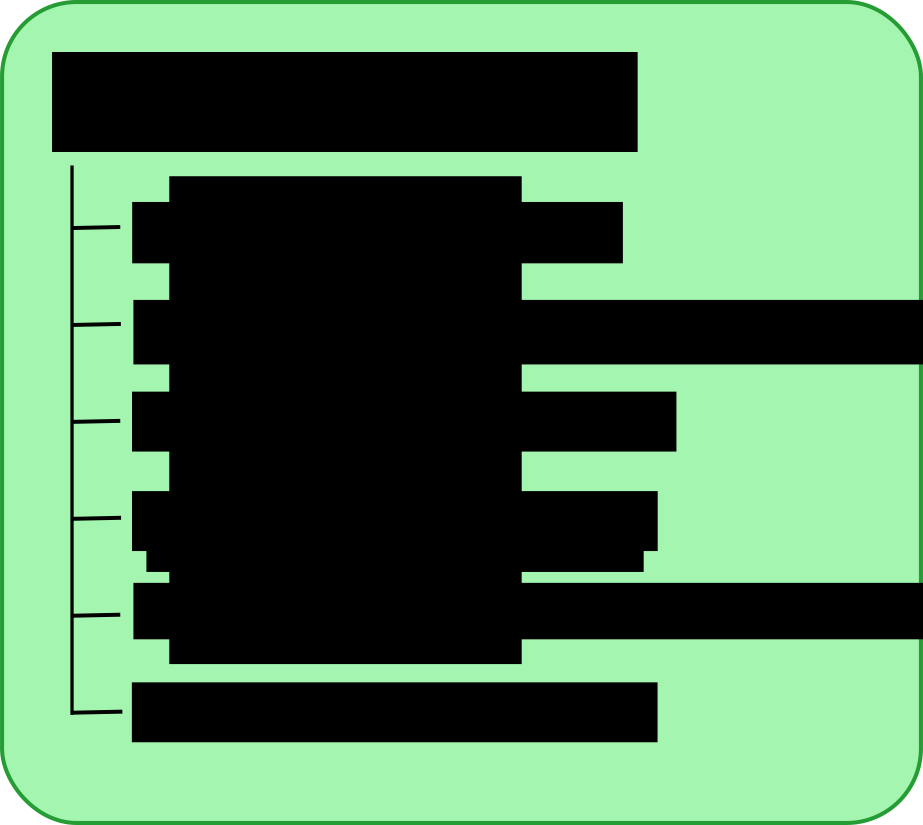
\includegraphics[width=0.9\linewidth]{neighborhood}
\caption{The methods all Neighborhood classes needs to implement.} 
\label{fig_neighborhood}
\end{figure} \noindent \noindent
All \class{Neighborhoods} implemented use a step function that changes value of a single independent variable, from 
0 to 1 or vise versa since all variables are binary. A neighborhood operation is stored in an a \class{Move} object 
that 
contains a pointer to the variable used, the variables change in value, and the change to the quality vector $Q$, 
once computed. The change in the quality vector is referred to at the \emph{delta vector}. \\ 
The \class{Neighborhood} classes that are implemented are shown in table \ref{tab_neighb}. \\  
\begin{table}[b]
\centering
\begin{tabular}{|l|l|}
\hline
class                          & Heuristic                                          \\ \hline
\class{FlipNeighborhood}     & All variables                                      \\ \hline
\class{RestrictedFlipNE}     & An expected 5000 variables chosen at random              \\ \hline
\class{ConflictOnlyNE}       & All variables in unsatisfied constraints           \\ \hline
\class{RandomConflictFlipNE} & Variables from a random unsatisfied constraint \\ \hline
\end{tabular}
\caption{Table of \class{Neighborhood} classes.}
\label{tab_neighb}
\end{table} \noindent
The method \method{next()} creates new \class{Move} object and returns a pointer to it. If all possible neighborhood 
operation of the neighborhood function have been returned the method returns a pointer to \textbf{NULL} instead. To know 
when  a neighborhood has been fully explored, counters and iterators are used depending on the neighborhood. These are 
reseted when returning \textbf{NULL} or the method \method{commitMove(move)} is called. The \class{Move} created only 
contain the variable and its suggested change in value, the delta vector is not computed yet. \\ 
For \class{FlipNeighborhood} when \method{next()} returns a \class{Move} and the variable chosen is given by a random 
sequence, a mask.  When \method{next()} is called in the \class{RestrictedFlipNE} class it returns the next variable 
probability $p = \frac{5000}{n}$, where $n$ is the number of independent variables. This gives expected 5000 variable 
before it return a \textbf{NULL} pointer. \\
For \class{ConflictOnlyNE} the neighborhood operations consist of a variable that participate in a constraint that is 
unsatisfied. \\ 
The class \class{RandomConflictFlipNE} chooses an unsatisfied constraint at random and returns a \class{Move} with 
a variable participating in that constraint until each \class{Move} with a different variable has been returned. \\
Method \method{nextRandom()} returns a \class{Move} with a random variable from the neighborhood.  \\ 
Method \method{calculateDelta(move)} takes a \class{Move} pointer as argument and propagate the change through the 
dependency digraph using the propagation queue of the variable. The method is identical for all the 
\class{Neighborhood} classes implemented. The method returns a flag that indicates if the suggested 
neighborhood operation is forbid by a oneway constraint. \\ 
The following describes how calculating the delta change of a variable $x_i$ changing value. 
\begin{enumerate} 
 \item Reset delta value of invariants in quality vector $Q$
 \item Send delta value of $x_i$ to neighbor invariants in DDG.
 \item For each invariant $y_j$ in propagation queue of $x_i$, calculate delta value $y_j$, if it is not zero, send 
the change to neighbors in DDG. 
 \item If a variables delta value is not allowed, by a oneway constraint, reset all delta values of invariant in 
the propagation queue. Then return false. 
 \item Otherwise update delta quality vector of move. 
\item return true if the $move$ is an allowed neighborhood operation. 
\end{enumerate} \noindent
The delta values of the invariants can be reset by calling \method{calculateDelta}, when no change is send. The 
reason for resetting them is only to make sure their stack of changes are empty before the next neighborhood operation 
is calculated. \\ 
To commit a neighborhood operation the method \method{commitMove(move)} is called with a pointer to the 
\class{Move} $move$ that is wanted. \method{commitMove(move)} recalculate the delta value 
by \method{calculateDelta(move)} since other neighborhood operation might have been explored since move was 
calculated last. Once the delta values of invariants have been computed, the invariants can be updated by calling their 
\method{updateValue()}. Invariants that represent violation of a single constraint are kept in a hash map of they are 
non zero. If they change value from non zero to zero or vise versa, that hash map needs to be updated. The hash map is 
used by the two neighborhoods \class{ConflictOnlyNE} and \class{RandomConflictFlipNE} that only can be used when the 
current solution is infeasible. If the current solution is feasible their neighborhood sizes are zero. \\
A default method \method{compareMoves(move1,move2)} compares the delta vector of two \class{Move} classes and 
returns 0 if they are the same, 1 if move1 is best and 2 otherwise. \\ 
The size of the neighborhood with the restriction applied to it, if any, can be requested from the 
method \method{getSize()}. It returns the size of the current neighborhood. For \class{ConflictOnlyNE} and 
\class{RandomConflictFlipNE} the neighborhood size can change after each iteration, for the others it is a constant 
size. \\ 

